\chapter{Forms of expressing information structure}
\label{chapter10-3}
\setcounter{enums}{0}

This chapter looks into specific forms of expressing information
structure in human language. Every language presumably has one or more
operations for articulating information structure. The operations are
strategized sometimes at the lexical level by employing specific
lexical items or rules, and sometimes at the phrasal level by using
special constructions.  Section \ref{10:ssec:focus-sensitive} goes over
\isi{focus} sensitive items, and presents how they are represented in
the articulation of information structure via \isi{ICONS} (Individual
CONStraints).\is{focus sensitive item}\is{Individual CONStraints}
Section \ref{10:sec:arg-opt} deals with argument optionality from the
perspective that focus is defined in terms of whether or not a
constituent is omissible (i.e.\ optionality).\is{argument optionality}
The remaining portion of the chapter addresses specific constructions
related to forming information structure.\is{argument optionality}
Section \ref{10:sec:scrambling} probes \isi{scrambling} behaviors in
\ili{Japanese} and \ili{Korean}, which are deeply related to the
arrangement of information structure components. Section \ref{10:sec:clefts}
delves into cleft constructions,\is{clefting} which are the most well
known operation for expressing focus in an overt way.
Section \ref{10:sec:passive} explores \isi{passive} constructions which play a
role in structuring of information in some languages.  Lastly,
Section \ref{10:sec:fronting} and Section \ref{10:sec:dislocation} investigate two
types of syntactic operations which are seemingly similar to each
other, but are constructed differently: focus/\isi{topic}
\isi{fronting} and \isi{dislocation}.



\section{Focus sensitive items}
\label{10:ssec:focus-sensitive}


\citet{lambrecht:96} provides several intriguing explanations
concerning the lexical properties of \isi{focus} sensitive
items.\is{focus sensitive item} First, emphatic reflexives cannot
involve a \isi{topic} interpretation, because they are usually focused
in the sentence. Second, NPIs (e.g.\ \textit{any} in English) and
negative words (e.g.\ \textit{not}, \textit{never}, \textit{no},
\textit{nobody}, \textit{nothing}, and so forth in English) cannot
play a topic role, for the same reason, either. This means that some
lexical categories, such as reflexives, NPIs, and negative words, are
inherently incompatible with the topic role. Nonetheless, focus
sensitive items do not all share the same properties.  Rather, there
are two subtypes of words with an inherent focus meaning. The nominal
elements, such as \textit{anybody}, \textit{nobody}, and
\textit{nothing}, are focus-sensitive by themselves. In contrast,
negative modifiers\is{negation} such as \textit{any}, \textit{not},
\textit{never}, and \textit{no} assign a focus relation not to
themselves, but to the constituent they modify. Henceforth, I call the
former Type I, and the latter Type II.


\myexe{\eenumsentence{\label{def:focus-sensitive:type}
\item{Focus Sensitive Type I assigns an information structure role
  (either \tdl{non-topic} or \tdl{focus}) to itself.}
\item{Focus Sensitive Type II assigns such a role to its adjacent
  constituent.}}}



\noindent Type I includes \textit{nothing}, \textit{nobody},
etc. These lexical items are contentful, introducing an EP into the
list of RELS. Their lexical constraint is inherited from
\tdl{one-icons-lex-item}, and additionally the TARGET of the element
on their \isi{ICONS} list is co-indexed with their INDEX.  Lexical
items under Type II also inherit from \tdl{one-icons-lex-item}, but
their TARGET is co-indexed with the INDEX of their modificands.  For
instance, a lexical entry for \textit{only} (Type II) can be described
as \myref{avm:only}. 

\myexe{\enumsentence{\label{avm:only}
\evnup{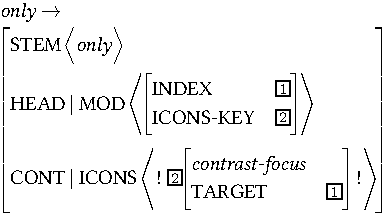
\includegraphics{pdf/only.pdf}}}}


\noindent Regarding the \tdl{info-str} value that \textit{only}
assigns to its modificands, it is specified as \tdl{contrast-focus} in
that \textit{only} has an exhaustive effect \citep{velleman:etal:12}.


The current analysis of the \isi{focus} sensitive particle \tdl{only} leaves
one central issue, which has to be left to further
research. \tdl{Only} in English needs not be adjacent to the focused
item that it is associated with. For example, in the following
sentence, \tdl{only} has an information structure relation to
\textsc{Kim} inside of the VP (A-accented).


\myexe{\enumsentence{\toplabel{exe:bild:only}
He only introduced \textsc{Kim} to Lee.}}


\noindent The current constraint presented in \myref{avm:only} cannot
handle this particular relation.  I leave it it to a future study to
find a way to link two non-adjacent individuals with respect to
information structure.


\subsection{Quantifiers}
\label{10:sssec:quantifiers}



Quantifiers  exhibit focus-sensitivity.\is{quantifier} In
particular, \citet{lambrecht:96} argues that universally quantified
NPs can be used as topics, whereas other quantified NPs cannot, as
exemplified in \myref{exe:lambrecht:quantifier}.\is{topic}


\myexe{\eenumsentence{\label{exe:lambrecht:quantifier}
\item{As for all his friends, they ...}
\item{*As for some people, they ... \citep[156]{lambrecht:96}}}}


\noindent That implies that non-universally quantifying determiners,
such as \textit{some}, assign \tdl{non-topic} to the head as
represented in \myref{avm:some}.



\myexe{\enumsentence{\label{avm:some}\evnup{
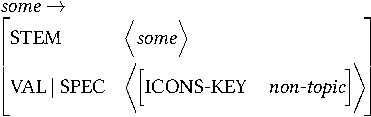
\includegraphics{pdf/some.pdf}}}}

\noindent In (\ref{exe:lambrecht:quantifier}b),\is{\textit{info-str}} what is responsible
for putting an \tdl{info-str} element into the \isi{ICONS} list is
\textit{as for} when we are not using the hypothetical suffixes \textit{-a}
and \textit{-b}.\is{quantifier} In this case, the \tdl{info-str} value of the element is
\tdl{topic}, the TARGET of the element is co-indexed with the INDEX of
\textit{people}, and the element itself is co-indexed with the
ICONS-KEY of \textit{people}.\is{ICONS-KEY} However, the ICONS-KEY of
\textit{people} is already constrained as \tdl{non-topic} by
\myref{avm:some}. Because this value is inconsistent with the
\tdl{topic} value introduced by \textit{as for}, \textit{as for some
  people} is ruled out.\is{topic}


\subsection{\textit{Wh}-words}
\label{10:sssec:wh}


\textit{Wh}-questions,\is{\textit{wh}-questions} as has been stated
many times so far, have been employed as a tool to probe the meaning
and markings of \isi{focus}: a technique which looks quite reliable
from a cross-linguistic stance.  \textit{Wh}-words have often been
regarded as inherently containing a focus meaning. That is to say, in
almost all human languages, \textit{wh}-words share nearly the same
distributional characteristics with focused words or phrases in
non-interrogative sentences.




A typological implication is provided in \citet[5]{drubig:03}: In a
language with \textit{wh}-phrases ex situ, the
\textit{wh}-phrase usually appears in \isi{focus} position. This
typological argument is convincingly supported by several previous
studies in which the linguistic similarity of \textit{wh}-words to
meaning and marking of focus is addressed.  According to
\citet{comrie:84} and \citet{buring:10}, \ili{Armenian} is a language
with strict focus position: Focused constituents should appear in the
immediately \isi{preverbal} position (as exemplified earlier in
Section \ref{4:sssec:preverbal}).  \citet{tamrazian:91} and
\citet{megerdoomian:11} argue that focused elements and
\textit{wh}-words in Armenian show a striking similarity to each other
from various points of view.\is{\textit{wh}-words} Tellingly,
\textit{wh}-words and focused constituents cannot co-occur, because
they occupy the same syntactic position.\is{syntactic positioning} In
other words, \textit{wh}-words should occur in the \isi{focus}
position in \ili{Armenian} (i.e.,\ in complementary distribution).



\myexe{\eenumsentence{\label{exe:hye:wh}
\item\shortex{4}
{ov & a & Ara-in & h{\textschwa}ravir-el?}
{who & \textsc{aux/3sg.pr} & Ara-\textsc{dat} & invite-\textsc{perf}}
{`Who has invited Ara'}
\item\shortexnt{5}
{*ov & Ara-in & a & h{\textschwa}ravir-el? & }
{who & Ara-\textsc{dat} & \textsc{aux/3sg.pr} & invite-\textsc{perf} & [hye]}
\item\shortexnt{5}
{*Ara-in & a & ov & h{\textschwa}ravir-el? &}
{Ara-\textsc{dat} & \textsc{aux/3sg.pr} & who & invite-\textsc{perf} & [hye] \citep{megerdoomian:11}}}}


\noindent According to the analysis of \citet{urbina:99},
\textit{wh}-words in \ili{Basque} are also in complementary distribution with focused
constituents in that both of them occupy the immediately
\isi{preverbal} position, optionally preceded by a constituent with
\isi{topic} meaning, and seldom occur in embedded clauses. Recall that the
canonical position of focused items in Basque is preverbal as
exemplified in Section \ref{4:sssec:preverbal} \mypage{exe:eus:joshua}.  From a
transformational perspective, \citet{urbina:99} argues that
\textit{wh}-words and focused items are able to undergo cyclic
movement with bridge verbs.



From these linguistic facts and analyses, the present study assumes
that \textit{wh}-words are inherently focused items which always have
a \tdl{focus} relation with the clause that they belong to. The
linguistic constraint on \textit{wh}-words is represented as the
following AVM. Note that \textit{wh}-words are \isi{focus sensitive}
items under Type I (\tdl{one-icons-lex-item}). The TARGET is
co-indexed with its INDEX.\is{focus sensitive item}\is{\textit{wh}-words}


\myexe{\enumsentence{\label{avm:wh-words}\evnup{
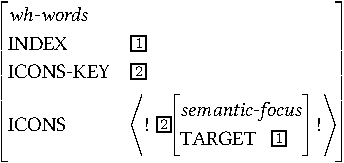
\includegraphics{pdf/wh-words.pdf}}}}


\myref{avm:wh-words} illustrates two more features of
\textit{wh}-words. First, as investigated in \citet{gryllia:09}
\textit{wh}-questions are incompatible with \isi{contrastive focus}.
The value of \isi{ICONS} should therefore be specified as
\tdl{semantic-focus}.\is{semantic focus} However, this does not
necessarily imply that the answer to a given \textit{wh}-question will
itself have \tdl{semantic-focus}.\is{\textit{wh}-question} As
discussed in Chapter~\ref{chapter3} (Section \ref{3:ssec:tests-contrast}), the
answerers may alter information structure in a solicited question as
they want, because \isi{contrastiveness} is heavily speaker-oriented
\citep{chang:02}.  The \onun-marked \textit{Kim-un} in
\myref{exe:kor:contrastive} delivers a contrastive
meaning,\is{contrast} but the answer does not directly correspond to
the question's information structure. Instead, the replier manipulates
information structure in order to attract a special attention to
\textit{Kim}. In other words, \textit{wh}-words themselves are still
assigned \tdl{semantic-focus} irrespective of the information
structure of the subsequent response.



\myexe{\eenumsentence{\label{exe:kor:contrastive:ch10-3}
\item[Q:]\shortex{2}
{nwuka & o-ass-ni?}
{who & come-\textsc{pst}-\textsc{int}}
{`Who came?' }
\item[A:]\shortex{2} 
  {Kim-un & o-ass-e.}
  {Kim-\textsc{nun} &  come-\textsc{pst}-\textsc{decl}}
  {`Kim came.'\\(conveying ``I know
  that at least Kim came, but I'm not sure whether or not others
  came.'') [kor]}}}



On the other hand, functionally speaking, there are two types of
interrogatives; informational questions and rhetorical questions. The
former explicitly solicits the hearer's reply, while the latter does
not. Since rhetorical questions perform a function of expressing an
assertion in a strong and paradoxical manner, their interpretation
naturally hinges on the context. For example, (\ref{exe:whocomes1}a)
can be ambiguously read as either an informational question or a
rhetorical question, and each reading can be paraphrased as
(\ref{exe:whocomes1}b--c), respectively. That means the
\textit{wh}-elements in rhetorical questions function like a trigger
to derive the form of interrogative sentences,\is{\textit{wh}-words}
but they can also convey quantificational readings as implied by
\textit{nobody} in (\ref{exe:whocomes1}c).\is{quantifier} In other
words, it is true that \textit{wh}-words convey \isi{focus} meaning in
\textit{wh}-questions, but not in all the sentential forms in which
they might appear.



\myexe{\eenumsentence{\label{exe:whocomes1}
\item Who comes?
\item I'm wondering which person comes.
\item Nobody comes.}}


Do all \textit{wh}-questions sound ambiguous (at least in
English)?\footnote{At the level of compositional semantics, rhetorical
  questions may not have to be considered in linguistic modeling,
  because they are basically a pragmatic phenomenon. What I want to
  say here is that other sentential constituents in
  \textit{wh}-questions can be focused, and this needs to be taken
  into account in modeling \textit{wh}-questions in a flexible
  way.\is{\textit{wh}-questions}} We know that in actual speech they
do not. This is because the meaning becomes unambiguous depending on
where the accent is assigned as illustrated in \myref{exe:whocomes2},
in which the A-accent falls on different words.


\myexe{\eenumsentence{\label{exe:whocomes2}
\item \textsc{Who} comes?\\
\ensuremath{\approx} I'm wondering which person comes.
\item Who \textsc{comes}?\\
\ensuremath{\approx} Nobody comes.}}


\noindent Informational questions, in order to clarify the meaning of
an assertion, employ an ordinary intonation pattern (i.e.\ rise-fall),
whereas rhetorical questions involve pitch accent within the
intonation contour \citep{gunlogson:01}. In other words, the prosodic
marking for information structure (i.e.\ intonation contour driven by
pitch accent) has an influence on the interpretation of
\isi{\textit{wh}-questions}. Note that \textit{comes} in
(\ref{exe:whocomes2}a) can be eliminated, while both \textit{who} and
\textsc{comes} are inomissible in (\ref{exe:whocomes2}b). The \isi{focus} in
(\ref{exe:whocomes2}b) comes from the accented verb \textsc{comes} and
spreads to the whole sentence (i.e.\ all-focus), whereby it forms a
different information structure from that of (\ref{exe:whocomes2}a).


If a \textit{wh}-question is rhetorically used, the entire sentence is
in the focus domain. For example, if \textit{Who comes?} is not asked
rhetorically, its information structure can be represented as
(\ref{fig:who-comes}a). The verb \textit{comes} in
(\ref{fig:who-comes}a) has \tdl{bg}, which implies that \textit{Who}
exclusively bears a \isi{focus} relation in the sentence. In contrast, if
the question is rhetorically used, the sentence should be
informatively structured as (\ref{fig:who-comes}b), in which the verb
\textit{comes} also has a \tdl{focus} relation within the clause
(i.e.\ \tdl{all-focus}). Since the choice between them is only
contextually conditioned, in an approach to \isi{grammar engineering}
that represents ambiguity via \isi{underspecification} wherever possible,
the MRS (\citealt{copestake:etal:05}) representing \textit{Who comes?} has
to be able to subsume (\ref{fig:who-comes}a--b).\is{MRS} Given that the
lowest supertype of \tdl{bg} and \tdl{focus} is \tdl{non-topic},
\textit{wh}-questions should be analyzed as
(\ref{fig:who-comes}c).\footnote{\tdl{Non-topic} on \textit{comes} in
  (\ref{fig:who-comes}c) should be introduced by a specific phrase
  structure rule to constrain \textit{wh}-questions with respect to
  information structure.  A creation of phrase structure rules for
  interrogative sentences is left to future work.}





\myexe{\enumsentence{\label{fig:who-comes}
\begin{tabular}[t]{llllllll}
a. & \evnup{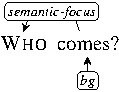
\includegraphics{pdf//who-comes-2.pdf}} & & b. &
\evnup{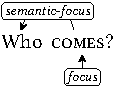
\includegraphics{pdf//who-comes-3.pdf}}  & & c. & 
\evnup{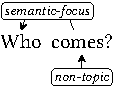
\includegraphics{pdf//who-comes-1.pdf}}  \\
\end{tabular}}}



\subsection{Negative expressions}
\label{10:sssec:neg}


Negation is sensitive to \isi{focus} \citep{partee:91,krifka:08}.\is{focus
  sensitive}\is{negation} For example, negative quantifiers
(e.g.\ \textit{no}),\is{quantifier} replacing sentential negation
(e.g.\ \textit{not ..., but ...}), and some other constructions
including negation such as \textit{neither ...} are associated with
focus almost invariably.  However, we cannot say negative verbs are
assigned \tdl{focus} all the time. For example, in the following Q/A
pair, the focused element should be the subject \textsc{Kim}. The rest
of the reply can be elided in the context.

\myexe{\eenumsentence{\label{exe:neg} 
\item[Q:]{Who didn't read the book?} 
\item[A:]{\textsc{Kim} (didn't read the book).}}}

\noindent For this reason, the present analysis argues that the value
that negative operators assign to operands is that of \tdl{non-topic},
which can be further resolved to \tdl{focus} or \tdl{bg} depending on
context.



\section{Argument optionality}
\label{10:sec:arg-opt}

Argument-optionality (also known as \textit{pro}-drop, including
\isi{subject-drop} and \isi{topic-drop}) has been assumed to be
related to information structure.\is{argument optionality} A basic
explanation of the relationship between dropped elements and
articulation of information structure is provided in
\citet{alonso:etal:02}, with special reference to subject-dropping in
\ili{Spanish}. Additionally, the distinction between subject-drop and
\isi{topic-drop} has also been studied in \citet{li:thompson:76},
\citet{huang:84} and \citet{yang:02} (as discussed in
Section \ref{3:sssec:inomissibility}).  Argument-optionality is also crucial
in computational linguistics; in multilingual processing, such as
(multilingual) anaphora resolution and machine translation
\citep{mitkov:etal:95,mitkov:99}, as well as in monolingual
processing, such as syntactic parsing and semantic
interpretation. Just as with other subfields of language processing,
there are two approaches to resolve dropped elements within language
applications: First, several rule-based algorithms have been designed
to resolve zero anaphora in \textit{pro}-drop
languages.\footnote{These are provided in \citet{han:06},
  \citet{byron:etal:06}, and so on.} Second, there are several
(semi-)machine-learning methods to compute zero anaphora in
\isi{topic-drop} languages for the purpose of machine
translation.\footnote{These can be found in \citet{zhao:ng:07},
  \citet{yeh:chen:04}, \citet{kong:ng:13}, and \citet{chen:ng:13} for
  Chinese, \citet{nakaiwa:shirai:96} and \citet{matsui:99} and
  \citet{hangyo:etal:13} for \ili{Japanese}, and \citet{roh:lee:03}
  for \ili{Korean}.}




In the present study, I use optionality and omissibility as
synonyms. Whether an argument can be elided or not needs to be
augmented into an analysis of argument optionality with respect to
focality.\is{argument optionality} As discussed thus far, the most
noteworthy feature of focused constituents is their inomissibility. If
a constituent is omitted then the constituent is not focused. This
restriction can be defined as \myref{def:focus:inomissibility}.  Note
that (\ref{def:focus:inomissibility}a) entails
(\ref{def:focus:inomissibility}b).\is{argument optionality}


\myexe{\eenumsentence{\label{def:focus:inomissibility}
\item C is inomissible iff C is focused. 
\item If C is omitted then C is not focused.}}


For example, \ili{Spanish} is a \isi{subject-drop} language.  The pronouns
are often missing as shown in
\myref{exe:sample:derivation:spa}. However, if they have a meaning of
\tdl{focus}, they have to appear with an accent
\citep{cinque:77,lambrecht:96}.  Therefore, the dropped subject in
\myref{exe:sample:derivation:spa} should be regarded as
\tdl{non-focus}.


\myexe{\enumsentence{\label{exe:sample:derivation:spa}
\shortex{2}
  {\O & Habla.}
  { & speaks}
  {`(He/She/It) speaks.' [spa]}}}


In the Argument Optionality library in the customization system
\citep{saleem:10,saleem:bender:10}, both subject dropping and object
dropping are described and modeled.\is{argument optionality}
The questionnaire requires users
to answer several questions; (i) whether or not subjects/objects can
be dropped in the user's language, (ii) whether or not the verb needs
to have a marker when the subjects/objects are dropped, (iii) whether
or not \isi{subject-drop} only happens in particular contexts, and (iv)
whether or not object-drop is lexically licensed.  To these potential
constraints, I add one more: Dropped elements are informatively
constrained as \tdl{non-focus}. This constraint should be written into
\tdl{basic-head-opt-subj-phrase} and \tdl{basic-head-opt-comp-phrase}.
These two phrasal types now include some additional constraints on
their subjects and complements as follows.



\myexe{\enumsentence{\label{avm:opt}
\begin{tabular}[t]{ll}
a. &  \evnup{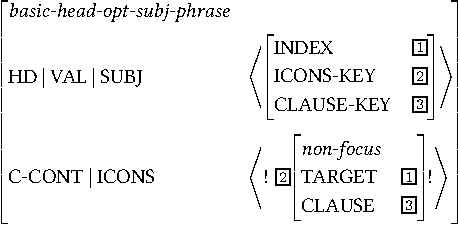
\includegraphics{pdf/basic-head-opt-subj-phrase.pdf}} \\
b. & \evnup{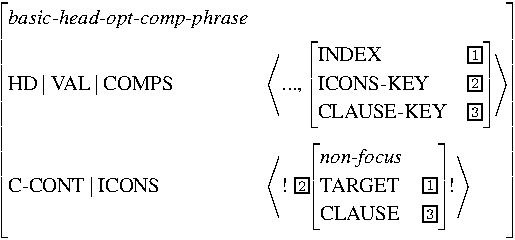
\includegraphics{pdf/basic-head-opt-comp-phrase.pdf}} \\
\end{tabular}}}


\noindent Building upon (\ref{avm:opt}a), the derivation tree for
\myref{exe:sample:derivation:spa} is sketched out in
\myref{fig:habla}.

\myexe{\enumsentence{\toplabel{fig:habla}
\begin{tabular}[t]{l}
\evnup{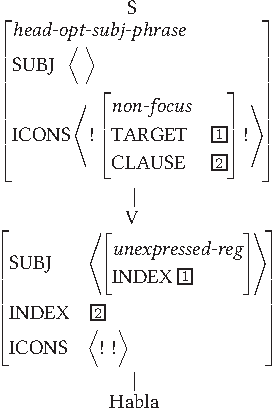
\includegraphics{pdf/habla.pdf}} \\
\end{tabular}}}



\section{Scrambling}
\label{10:sec:scrambling}


The typical case in which forms of expressing information structure do
not coincide with information structure meanings can be found in the
use of \wa in \ili{Japanese} and \nun in \ili{Korean}.\is{scrambling}
NPs in Japanese and Korean, as presented several times, can have three
types of marking; case-marking, \wa or \onun-marking, and null-marking
(also known as case ellipsis). These are in
complementary distribution with each other, and the choice among them
is largely conditioned by information structure.

\myexe{\enumsentence{\label{exe:np-marking:jpn} 
\shortex{2} 
{Kim-ga/wa/\O & kita.}
{Kim-\textsc{nom}/\textsc{wa}/\textsc{null} & came}
{`Kim came. [jpn]'}}}


\noindent As stated before, \wa and \nun can convey meaning of
aboutness topic,\is{aboutness topic} contrastive topic, or even contrastive
focus \citep{choi:99,song:bender:11}.\footnote{In this vein, 
\wa and \nun perform the same role as the
  B-accent in English, which can also be used to express
  \isi{non-contrastive topic}, \isi{contrastive topic},
  or sometimes \isi{contrastive focus} \citep{hedberg:06}.}  Case
markers are also ambiguously interpreted.  They have sometimes been
assumed to be associated with \isi{focus}, but there are quite a few
counterexamples which show that all case-marked NPs do not necessarily
convey focus meaning in all languages \citep{heycock:94}. Null-marking
is also conditioned by information structure in some languages: The
markers are not omissible if an NP is associated with \tdl{focus},
which means that the null-marked NPs receive an interpretation of
either topic or \isi{background} (i.e.\ \tdl{non-focus}).\is{topic}


Nevertheless, this does not mean that NPs in \ili{Japanese} and
\ili{Korean} deliver an informatively knotty meaning all the time. The
meanings can be disentangled at the phrasal level, mainly via
different word orders, such as basic \vs scrambling.\is{scrambling}
Scrambling refers to constructions in which one or two objects are
followed by the subject. This construction is productively used in
Japanese and Korean (i.e.\ SOV in the basic order \vs OSV in the
scrambled order). Scrambling has been rather discounted as a dummy
operation in syntax and semantics, but \citet{choi:99} and
\citet{ishihara:01} argue that scrambling has a strong effect on
information structure.  The contrast between orders with respect to
\wa is exhibited in the following examples.\footnote{There can be one
  more sentence from this paradigm though \citet{maki:etal:99} do not
  include it in their source; \textit{Kono hon-o John-wa yonda}, which
  is completely grammatical, but the \wa-marked \textit{John} is
  interpreted as indicating \isi{contrastiveness}. In order to show the
  authors' example as is, this sentence is not included in
  \myref{exe:maki:7-8:ch10-3}.}




\myexe{\eenumsentence{\label{exe:maki:7-8:ch10-3}
\item\shortex{4}
{John-wa & kono & hon-o & yonda.}
{John-\textsc{wa} & this & book-\textsc{acc} & read}
{`As for John, he read this book.'}
\item\shortex{4}
{Kono & hon-wa & John-ga & yonda.}
{this & book-\textsc{wa} & John-\textsc{nom} & read}
{`As for this book, John read it.'}
\item\shortex{4}
{John-ga & kono & hon-wa & yonda.}
{John-\textsc{nom} & this & book-\textsc{wa} & read}
{`John read this book, as opposed to some other book.' \\
`*As for this book, he read this it.' [jpn] \citep[7--8]{maki:etal:99}}}}



\noindent The first sentence is in the \isi{basic word order}, in
which the subject is topicalized. The second sentence is scrambled,
and the fronted object carries a \isi{topic} meaning
(i.e.\ \tdl{contrast-topic}). The third sentence is in the basic word
order, but \wa is attached to the object, not the subject. In that
case, the topicalized object should be interpreted as containing
\isi{contrastiveness} (i.e.\ \tdl{contrast-focus}). Regarding the
relationship between \wa or \onun-marking and word-order in
\ili{Japanese} and \ili{Korean}, \citet{song:bender:11} provide
Table~\ref{tbl:top}, adapted from \citet{choi:99}.




\begin{table}[h]
\caption{Information structure of \onun-marked NP}
\centering
\begin{tabular}{|c|c|c|}
\hline
& \textbf{in-situ} & \textbf{scrambling} \\
\hline
\textbf{subject} & \tdl{topic} & \tdl{contrast-focus} \\
\hline
\textbf{non-subject} & \tdl{contrast-focus} & \tdl{contrast-topic} \\ 
\hline
\end{tabular}
\label{tbl:top}
\end{table}


According to Table~\ref{tbl:top}, the set of allosentences given in
\myref{exe:yomu} have different information structure.  In other
words, the default meaning of \wa and \nun
(i.e.\ \tdl{contrast-or-topic}) can be narrowed down, through
interaction with word order (e.g.\ scrambling).\is{scrambling}




\myexe{\eenumsentence{\toplabel{exe:yomu}
\item\shortexnt{6}
{Kim & wa & sono & hon & o & yomu.}
{Kim & \textsc{wa} & \textsc{det} & book & \textsc{acc} & read (\tdl{topic})}
\item\shortexnt{6}
{sono & hon & o & Kim & wa & yomu.}
{\textsc{det} & book & \textsc{acc} & Kim & \textsc{wa} & read (\tdl{contrast-focus})}
\item\shortexnt{6}
{Kim & ga & sono & hon & wa & yomu.}
{Kim & \textsc{nom} & \textsc{det} & book & \textsc{wa} & read (\tdl{contrast-focus})}
\item\shortexnt{6}
{sono & hon & wa & Kim & ga & yomu.}
{\textsc{det} & book & \textsc{wa} & Kim & \textsc{nom} & read (\tdl{contrast-topic}) [jpn]}}}

\noindent There is one additional property that \wa and \nun display:
They cannot appear in an \tdl{all-focus} construction that allows only
\tdl{semantic-focus} lacking contrastive meanings, as exemplified in
\myref{exe:wa:all-focus}.\is{contrast}\is{semantic focus}


\myexe{\eenumsentence{\toplabel{exe:wa:all-focus}
\item[Q:]\shortex{2}
{doushita & nano}
{what & \textsc{int}}
{`What happened?'}
\item[A:]\shortex{6}
  {Kim & ga/\#wa & sono & hon & o/\#wa & yabut-ta.}
  {Kim & \textsc{nom}/\textsc{wa} & \textsc{det} & book & \textsc{acc}/\textsc{wa} & tear-\textsc{pst}}
  {`Kim tore the book.' [jpn]}}}

In syntactic derivation, \tdl{topic-comment} presented below plays an
important role in creating grammatical rules.\is{topic-comment} The
construction itself is \mbox{[MKG \tdl{tp}]} so that constituents
which have picked up a \isi{topic} cannot serve as the head daughter
of another \tdl{topic-comment} phrase.\is{MKG}

\myexe{\enumsentence{\label{avm:topic-comment:3}
\evnup{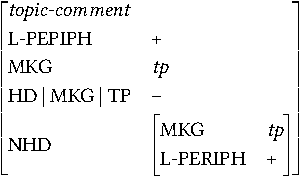
\includegraphics{pdf/topic-comment3.pdf}}}}



\noindent The phrasal rules, such as \tdl{subj-head-rule} and
\tdl{comp-head-rule}, are classified into subrules, which inherit from
two types of head-phrases (i.e. \tdl{subj-head-phrase} and
\tdl{comp-head-phrase}) and optionally \tdl{topic-comment}.\is{topic-comment} This type
hierarchy is presented in Figure~\ref{fig:top:scr}, in which there are
two factors that have an influence on branching nodes; \wa or
\onun-marking (i.e.\ \tdl{top-}) and scrambling (i.e.\ \tdl{scr-}).


\begin{figure}[!t]
\begin{center} 
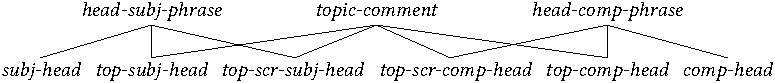
\includegraphics[width=.9\textwidth]{pdf/top-scr.pdf}
\caption{Phrase structure rules of scrambling in Japanese and Korean}
\label{fig:top:scr}
\end{center}
\end{figure}


This tripartite strategy is potentially controversial in that several
types of headed rules are introduced. In the spirit of HPSG,\is{HPSG}
reducing the number of rules should be considered in order to avoid
redundancy. From this point of view, the six grammatical rules
presented in Figure~\ref{fig:top:scr} might look rather superfluous.
Nevertheless, the present model pursues this strategy for several
reasons. First, \ili{Japanese} and \ili{Korean} are typical
topic-prominent languages in which expressing topics plays an
important role in configuring sentences
\citep{li:thompson:76,sohn:01}.\is{topic-comment} Accordingly, it is my belief that the
use of \tdl{topic-comment} as one of the major phrase structure types
is never ill-conceived in creating Japanese and Korean
grammars. Second, if we did not refer to the marking system
(i.e.\ MKG),\is{MKG} we would allow too wide an interpretation of
scrambled constructions.\is{topic} That is, it would be almost impossible to
narrow down the information structure meaning that \wa and \nun
inherently carry (i.e.\ \tdl{contrast-or-topic}), if it were not for
such discrimination.  One alternative analysis would be to treat
topicalized and scrambled constituents as a \tdl{head-filler-phrase}.
However, this is poorly suited to handling scrambling.  Such a
\tdl{head-filler}-based analysis predicts the creation of a
long-distance dependency (i.e.\ scrambling across clause
boundaries),\is{scrambling} but such a dependency is unlikely to
occur. Furthermore, the basic \tdl{head-comp} and \tdl{head-subj}
properties are still encoded in single types, and these types are
cross-classified with others to give the more specific rules. That
means that there are no missing generalizations.  It seems clear that
the tripartite strategy is well-motivated and is the most effective
way to manipulate information structure in Japanese and Korean.



More specific information structure values are assigned by each
grammatical rule, adding constraints to both HEAD-DTR and
NON-HEAD-DTR. For example, \tdl{top-scr-subj-head} and
\tdl{top-scr-comp-head} impose a value on NON-HEAD-DTR as shown in
\myref{avm:top:scr}.\footnote{ICONS-KEY is doing some valuable work
  here,\is{ICONS-KEY} because it lets both the phrase structure rules
  and the lexical rules/entries contribute partial information to the
  same \isi{ICONS} element.}


\myexe{\enumsentence{\label{avm:top:scr}
\begin{tabular}[t]{ll}
a. & \evnup{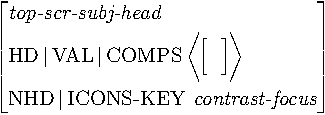
\includegraphics{pdf/top-scr-subj-head.pdf}}\\
b. & \evnup{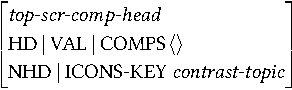
\includegraphics{pdf/top-scr-comp-head.pdf}} \\
\end{tabular}}}


\noindent On the other hand, grammatical rules whose NON-HEAD-DTR is
non-topicalized (e.g.\ \tdl{subj-head} and \tdl{comp-head}) constrain
the NON-HEAD-DTR to be [MKG{$\mid$}TP \tdl{na-or-${-}$}], and the
information structure values (i.e.\ ICONS-KEY)\is{MKG}\is{ICONS-KEY}
comes from the lexical information provided by case markers
(i.e.\ \tdl{non-topic}) and the null marker
(i.e.\ \tdl{non-focus}). Consequently, the parse trees and dependency
graphs for (\ref{exe:yomu}b) and (\ref{exe:yomu}d) are illustrated in
\myref{fig:sono-hon-o-kim-wa-yomu} and
\myref{fig:sono-hon-wa-kim-ga-yomu}, respectively.

\myexe{\eenumsentence{\label{fig:sono-hon-o-kim-wa-yomu}
\item\evnup{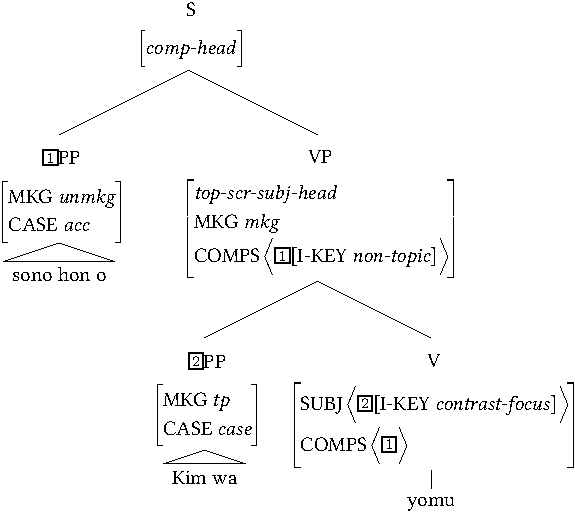
\includegraphics{pdf/sono-hon-o-kim-wa-yomu-tree.pdf}}
\item\evnup{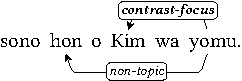
\includegraphics{pdf/sono-hon-o-kim-wa-yomu.pdf}}}}


\noindent In (\ref{fig:sono-hon-o-kim-wa-yomu}a), the \wa-marked
subject \textit{Kim} is combined with the verb \textit{yomu}
`read'.\footnote{The reason why \textit{sono hon o}/\textit{wa} and
  \textit{Kim ga}/\textit{wa} are labeled as PPs, not NPs is given in
  \citet{yatabe:99} and \citet{siegel:99}.} This combination is an
instance of \tdl{top-scr-subj-head} which requires \mbox{[MKG
    \tdl{tp}]} of the NON-HEAD-DTR (i.e.\ \textit{Kim wa}) and assigns
\tdl{contrast-focus} to the ICONS-KEY of the NON-HEAD-DTR. Since there
is no specific constraint on MKG in this phrase structure, the value
of MKG remains underspecified
(i.e.\ \tdl{mkg}).\is{ICONS-KEY}\is{\textit{mkg}} Next, the VP takes
\textit{sono hon o} `the book' as its complement. Because the fronted
object is not \wa-marked, its information structure meaning is still
represented as \tdl{non-topic}, which comes from the case-marking
adposition \textit{o} `\textsc{acc}'.\is{adposition}

\myexe{\eenumsentence{\label{fig:sono-hon-wa-kim-ga-yomu}
\item\evnup{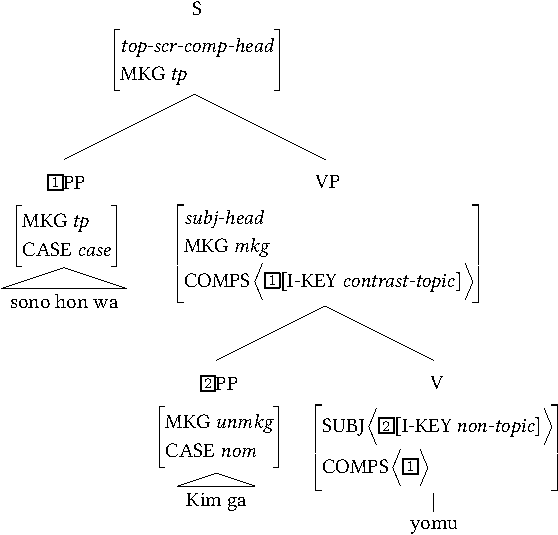
\includegraphics{pdf/sono-hon-wa-kim-ga-yomu-tree.pdf}}
\item\evnup{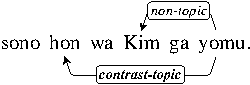
\includegraphics{pdf/sono-hon-wa-kim-ga-yomu.pdf}}}}


\noindent On the other hand, since the scrambled object in
(\ref{fig:sono-hon-wa-kim-ga-yomu}a) is {\wa}-marked, the top node is
an instance of \tdl{top-scr-comp-head}, which assigns
\tdl{contrast-topic} to the complement. Thus, \isi{topic} falls on the
object, while the case-marked subject conveys \tdl{non-topic}.


To summarize,\is{scrambling}\is{lexical markers} scrambling in
\ili{Japanese} and \ili{Korean} has to do with both lexical markers
(e.g.\ \wa and \nun) and constraints on
\tdl{topic-comment}.\is{topic-comment} In order to systematize the
different values that scrambled arguments and non-scrambled arguments
have with respect to information structure, the present study proposes
a tripartite strategy using cross-classification of three phrase
structure types: \tdl{head-subj-phrase}, \tdl{head-comp-phrase}, and
\tdl{topic-comment}.\is{MKG} \mbox{[MKG \tdl{tp}]} is used to control
the combination of the different phrase structure rules (and lexical
markers) so that the scrambled and non-scrambled versions can be
detected and related to their appropriate \textit{info-str}
values.\is{\textit{info-str}}



\section{Cleft constructions}
\label{10:sec:clefts}


Clefting is a special syntactic operation expressing \isi{focus} in a marked
way.\is{clefting} Quite a few languages, including English, have the
focus-related syntactic device called cleft constructions.  All
languages have at least one way to express focus, but it is unlikely
that all languages have cleft constructions.


Cleft constructions normally involve relative clauses,\is{relative
  clause} which are not yet implemented in the \lingo \isi{Grammar
  Matrix} system.  For these reasons, clefts are not included within
the information structure grammar library for the customization system
(Chapter~\ref{chapter11}).  This section, instead, deals with how
cleft constructions are analyzed within the HPSG/MRS formalism on a
theoretical basis with special reference to \isi{ERG} (English Resource
Grammar, \citealt{flickinger:00}).



\subsection{Properties}
\label{10:sssec:clefts:properties}



Cleft constructions are regarded as showing different behaviors from
ordinary focused constructions in syntax as well as semantics.\is{clefting} In a
nutshell, clefts are associated with exhaustive \isi{focus}, which renders
(\ref{exe:clefts:velleman}b) infelicitous.

\myexe{\eenumsentence{\label{exe:clefts:velleman}
\item{\textsc{John} laughed, and so did \textsc{Mary}.}
\item{\#It was \textsc{John} who laughed, and so did
  \textsc{Mary}. \citep[444]{velleman:etal:12}}}}

\noindent \citet{kim:12a}, in a similar vein, argues clefts cannot
coincide with lexical items that conflict with exhaustive focus. For
example, \textit{even} cannot be used in the focused XPs of cleft
constructions as exemplified below.

\myexe{\enumsentence{\label{exe:clefts:kim}
{*It was even the advanced textbook that the student
  read. \citep[48]{kim:12a}}}}


\noindent However, not all identificational foci are always realized
as cleft constructions.\is{clefting} Identificational foci can be
conveyed in some languages using marked word order, as exemplified in
the examples in Hungarian (\ref{exe:kiss:ch10-3}a) and Standard Arabic
(\ref{exe:arabic:ch10-3}a).  That is, clefting is a sufficient
condition for expressing identificational \isi{focus}, but not a necessary
one.



\myexe{\enumsentence{\label{exe:kiss:ch10-3}
\shortex{6} 
{Mari & \textsc{egy} & \textsc{kalapot} & n\'{e}zett & ki & mag\'{a}nak.}
{Mary & a & hat.\textsc{acc} & picked & out & herself.\textsc{acc}}
{`It was \textsc{a hat} that Mary picked for herself.' [hun] \citep[249]{kiss:98}}}}

\myexe{\enumsentence{\label{exe:arabic:ch10-3}
\shortex{3}
  {RIWAAYAT-AN & {\textglotstop}allat-at & Zaynab-u}
  {novel-\textsc{acc} & wrote-she & Zaynab-\textsc{nom}}
  {`It was a \textsc{novel} that Zaynab wrote.' [arb] \citep[337]{ouhalla:99}}}}




In addition to the semantic differences, Hungarian clefts also 
exhibit distinct prosodic patterns as shown in \myref{exe:kiss:ch10-3}.  
\citet{gussenhoven:07} offers an analysis of cleft
constructions in English with respect to information status.  The
clefted and non-clefted constituents are optionally accented.  If the
non-clefted constituent is accented, then clefts cause the non-clefted
constituent to be interpreted as reactivated information (as presented
in the first pair of
\ref{exe:gussenhoven:clefts:ch10-3}).\footnote{\citet{gussenhoven:07}
  argues that the first reply in
  \myref{exe:gussenhoven:clefts:ch10-3:here} implies Helen's disfavor
  to somebody had been discussed recently.}  On the other hand, if the
non-clefted constituent is unaccented, and the clefted one bears the
accent as given in the second pair of
\myref{exe:gussenhoven:clefts:ch10-3:here}, the clefted and
non-clefted part denote new/old information, respectively. It is
impossible to have both clefted and non-clefted constituents deliver
new information at the same time.

\myexe{\eenumsentence{\label{exe:gussenhoven:clefts:ch10-3:here}
\item[Q:]{Does Helen know \textsc{John}?} 
\item[A:]{It is John/\textsc{John} she \textsc{dislikes}.}
\item[Q:]{I wonder who she dislikes.} 
\item[A:]{It is \textsc{John} she dislikes. \citep[96]{gussenhoven:07}}}}


\subsection{Subtypes}
\label{10:sssec:clefts:subtypes}


Clefts\is{clefting} can be classified into subtypes.\footnote{From a
  functional perspective, \citet{kim:yang:09} classify cleft
  constructions into predicational, identificational, and eventual
  types.  Similarly \citet{clech:99} classify cleft constructions in
  \ili{French} (basically realized in the form as \textit{C'est ... que/qui
    ...})  into four types: basic, broad event-related \isi{focus}, broad
  presentational focus, exclamatory comment. This taxonomy is not used
  in the current analysis.}  These include \textit{it}-clefts,
\textit{wh}-clefts (also known as pseudo clefts), and inverted
\textit{wh}-clefts \citep{kim:07}.  Each of them is exemplified in
\myref{exe:kim:07}, whose skeletons are represented in
\myref{exe:kim:07:skeleton} in turn.\footnote{(\ref{exe:kim:07}a) is
  originally taken from the ICE-GB corpus (\citealt{nelson:etal:02}),
  and the bracketed expression after the sentence stands for the
  indexing number. (\ref{exe:kim:07}a) is paraphrased into
  (\ref{exe:kim:07}b--c) by \citet{kim:07}.}


\myexe{\eenumsentence{\label{exe:kim:07}
\item{\textit{It}-clefts: In fact it's their teaching material that we're using... \ensuremath{<}S1A-024 \#68:1:B\ensuremath{>}}
\item{\textit{Wh}-clefts: What we're using is their teaching material.}
\item{Inverted \textit{wh}-clefts: Their teaching material is what we are using. \citep[217]{kim:07}}}}
\myexe{\eenumsentence{\label{exe:kim:07:skeleton}
\item{\textit{It}-clefts: It + be + XP\mysub{i} + cleft clause}
\item{\textit{Wh}-clefts: Cleft clause + be + XP\mysub{i}}
\item{Inverted \textit{wh}-clefts: XP\mysub{i} + be + cleft clause \citep[218]{kim:07}}}}


\noindent \citet{kim:07}, building upon this taxonomy, provides a
corpus study with reference to ICE-GB (a syntactically annotated
corpus of British English, \citealt{nelson:etal:02}). Out of 88,357
sentences in the corpus, \textit{it}-clefts occur 422 times (0.47\%),
\textit{wh}-clefts occur 544 times (0.61\%), and inverted
\textit{wh}-clefts occur 537 times (0.60\%). In addition to NPs,
various phrasal categories can be focused in cleft
constructions. These include APs, AdvPs, PPs, VPs, and even CPs. For
example, \textit{it}-clefts can take various types of XPs as the
focused constituent.


\myexe{\eenumsentence{\label{exe:xp:cleft:kim:07}
\item{NP: It was [the gauge] that was the killer in the first
  place. \ensuremath{<}S1A-010 \#126:1:B\ensuremath{>}}
\item{AdvP: And it was [then] that he felt a sharp
  pain. \ensuremath{<}S2A-067 \#68:1:A\ensuremath{>}}
\item{Subordinate Clause: It wasn't [till I was perhaps twenty-five or
    thirty] that I read them and enjoyed them \ensuremath{<}S1A-013
  \#238:1:E\ensuremath{>} \citep[220]{kim:07}}}}



\noindent One interesting point is that there is a restriction on
categorical choice. \citet[220--223]{kim:07} presents the
frequency as shown in Table~\ref{tbl:freq:cleft}.


\begin{table}[!h]
\caption{Frequency of the three types of clefts \citep{kim:07}}   
\centering
\begin{tabular}{|l||r|r|r|r|r|r|}
\hline
Types of XP & NP & AP & AdvP & PP & VP & CP \\
\hline
\textit{it}-cleft & 324 & 0 & 18 & 65 & 0 & 16 \\
\hline
\textit{wh}-cleft & 136 & 19 & 3 & 14 & 19 & 275 \\
\hline
inverted \textit{wh}-cleft & 518 & 0 & 0 & 0 & 0 & 19 \\
\hline
\end{tabular}
\label{tbl:freq:cleft}
\end{table}

Table~\ref{tbl:freq:cleft} shows the following:\is{clefting} \textit{It}-clefts
seldom take verbal items as the pivot XP, while \textit{wh}-clefts do
not show such a restriction.  Inverted \textit{wh}-clefts exclusively
put \isi{focus} on NPs, but there are some exceptional cases in which the
focused constituent is clausal as exemplified below.



\myexe{\eenumsentence{\label{exe:cp:cleft:kim:07}
\item{[To feel something you have written has reached someone] is what
  matters. \ensuremath{<}S1A-044 \#096\ensuremath{>}}
\item{[What one wonders] is what went on in his
  mind. \ensuremath{<}S1A-044 \#096\ensuremath{>} \citep[222]{kim:07}}}}


\noindent Though various types of phrases can be focused in clefts,
\citet{velleman:etal:12} argues that only a portion of the pivot is
assigned genuine \isi{focus}. This implies that clefts involve narrowly
focused items inside of the pivot XP as \citet{beaver:clark:08} argue
that the clefts raise an exhaustive reading as a \isi{focus sensitive operator}.\is{narrow focus}



The present analysis is exclusively concerned with \textit{it}-clefts,
basically following the analysis provided by the \isi{ERG}.  Implementing
\textit{it}-clefts in \isi{TDL} (Type Description Language)
requires a categorical constraint indicated
in Table~\ref{tbl:freq:cleft}: non-clausal verbal items are not used
as the pivot XPs.  Pseudo cleft constructions, such as
\textit{wh}-clefts and inverted \textit{wh}-clefts, are left to future
work, because free relative clauses need to be separately implemented
in relation to ICONS.


\subsection{Components}
\label{10:sssec:clefts:components}

Cleft constructions across languages are made up of four components
\citep{gundel:02,kim:yang:09,kim:12a};  placeholder,  copula,
pivot XP, and cleft clause.\is{copula}\is{clefting}


\myexe{\enumsentence{\label{exe:cleft:component}
\shortexnt{4}
{[It] & [is] & [the dog] & [that barks].}
{placeholder & copula & pivot XP & cleft clause}}}




\noindent Some languages constitute cleft constructions in the same
way as English.  For instance, a basic cleft sentence
\myref{exe:cleft:nor} in \ili{Norwegian} is comprised of all the four
components.

\myexe{\enumsentence{\label{exe:cleft:nor}
\shortexnt{5}
{Det & var & Nielsen & som & vant.}
{It & was & Nielsen & that & won [nor] \citep[113]{gundel:02}}}}

\noindent However, the first two components are not necessarily used
in all languages that employ clefts. The following subsections explore
these four components in turn.



\subsubsection{Placeholders}
\label{10:sssec:clefts:placeholders}


For English,\is{clefting} placeholders in cleft constructions are
usually realized as expletives (i.e.\ \textit{it} in English)
\citep{pollard:sag:94}, but some counterexamples to this
generalization exist. \citet{kim:12a} presents a dialogue in which
\textit{it} in a cleft construction is made use of as a referential
pronoun, rather than an expletive. \citet{ han:hedberg:08} exemplify a
specific context in which demonstrative pronouns (e.g.\ \textit{this}
and \textit{that}) can be substituted for \textit{it}. Moreover, some
languages do not employ any placeholder. For example, clefts in Arabic
languages and in \ili{Wolof} (a Niger-Congo language, spoken in
Senegal) have no counterpart to \textit{it}. In the following examples
(\ili{Standard Arabic} in (\ref{exe:cleft:arb}a), \ili{Moroccan
  Arabic} in (\ref{exe:cleft:arb}b), and \ili{Wolof} in
\ref{exe:cleft:arb}c), the focused constituents occupy the first
position of the sentence, followed by pronominal copulae, such as
\textit{hiyya} in (\ref{exe:cleft:arb}a) and \textit{huma} in
(\ref{exe:cleft:arb}b) or an ordinary copula \textit{la} in
(\ref{exe:cleft:arb}c), and then followed by cleft clauses.



\myexe{\eenumsentence{\label{exe:cleft:arb}
\item\shortex{5}
{ZAYNAB-u & hiyya & llatii & {\textglotstop}allaf-at & l-riwaayat-a.}
{Zaynab-\textsc{nom} & \textsc{pron}.she & \textsc{rm} & wrote-she & the-novel-\textsc{acc}}
{`It was ZAYNAB who wrote the novel.' [arb]}
\item\shortex{6}
{L-WLAD & huma & Hi & sarrd-at & (-hum) & Nadia.}
{the-children & \textsc{pron}.they &  \textsc{rm} & sent-she & (-them) & Nadia}
{`It was the CHILDREN that Nadia sent.' [ary] \citep[341]{ouhalla:99}}
\item\shortex{6}
{Fas & wi & la & jaakat & bi & j\"end}
{horse & the & \textsc{cop.3sg} & merchant & the & buy}
{`It is the horse (that) the merchant bought.' [wol] \citep[256]{kihm:99}}}}

\noindent This current model assumes that the placeholder for clefts is
conditioned language-specifically. As for the placeholder \textit{it}
in English clefts, it is assumed to be a semantically vacuous pronoun
(i.e.\ an expletive) that introduces no EP and involves an empty ICONS
list (i.e.\ \tdl{no-icons-lex-item}).


\subsubsection{Copulae}
\label{10:sssec:clefts:cop}


Copulae participate in cleft constructions.  However, not all
languages employ copulae, and the use of copulae is
language-specific. For example, \ili{Russian} does not use any copula
in clefts, as exemplified below.\is{copula}

\myexe{\enumsentence{\label{exe:cleft:rus}
\shortex{5}
{Eto & [Boris] & vypil & vodku.}
{it	& Boris	& drank	& vodka}
{`It is Boris-\textsc{foc} (who) drank the vodka.' [rus] \citep[80]{king:95}}}}


\noindent Thus, (ii) the use of a copula is not a mandatory
cross-linguistic component for constructing clefts.\is{copula}


On the other hand, it is necessary to determine the grammatical status
of the copulae in clefts.\is{copula} \citet{kim:12a} surveys two
traditional approaches to cleft constructions: (a) extraposition
\citep{gundel:77} and (b) expletive \citep{kiss:99,lambrecht:01}.
First, the extraposition analysis assumes \textit{it}-clefts stem from
\textit{wh}-clefts;\is{relative clause} a free relative clause in a
\textit{wh}-cleft construction is first extraposed
(i.e.\ right-dislocated) leaving \textit{it} in the basic position,
and then \textit{what} in the extraposed clause turns into an ordinary
relative pronoun such as \textit{that}.  Second, the expletive
analysis assumes that the pronoun \textit{it} is a genuine expletive
(i.e.\ generated in situ), and the cleft clause is directly
associated with the pivot XP. For example, a simple cleft sentence
\textit{It is the dog that barks.}  can be parsed into
(\ref{exe:erg:vs:kim}a--b) respectively. In (\ref{exe:erg:vs:kim}a),
the copula \textit{is} takes two complements; one is the pivot XP
\textit{the dog}, and the other is the cleft clause \textit{that
  barks}. In contrast, the copula in (\ref{exe:erg:vs:kim}b) takes
only one complement, and the pivot XP and the cleft clause are
combined with each other before being dominated by the copula.


\myexe{\eenumsentence{\label{exe:erg:vs:kim}
\item{[It [[\mysub{\textsc{head-dtr}} is the dog] [\mysub{\textsc{non-head-dtr}} that barks]]].}
\item{[It [is [[\mysub{\textsc{head-dtr}} the dog] [\mysub{\textsc{non-head-dtr}} that barks]]]].}}}


\noindent \citeauthor{kim:12a} provides a hybrid approach between the
extraposition analysis and the expletive analysis.\is{clefting} For him, the
focused XP constitutes a \tdl{cleft-cx} with the following cleft
clause first, and then the copula takes the \tdl{cleft-cx} as a single
complement. That is, his analysis takes (\ref{exe:erg:vs:kim}b) as the
proper derivation of the cleft sentence.


The \isi{ERG} parses a cleft sentence similarly to the extraposition
analysis; along the lines of the parse in
(\ref{exe:erg:vs:kim}a). That is, in the ERG analysis of
\textit{it}-clefts the focused XP complements the copula, and the
construction introduces a constructional content structure
(i.e.\ C-CONT) whose EP is ``\_be\_v\_itclefts\_rel'', and then the VP
(i.e.\ [copula + XP]) is complemented once again by cleft
clauses. This follows the traditional approach in which the copula in
clefts takes two complements; one for the focused constituent, and the
other for the cleft clause.




On one hand, the two HPSG-based analyses both treat the copula in
clefts as a single entry, lexically different from ordinary
copulae. On the other hand, they differ with respect to the ARG-ST
values of the cleft copula.\is{copula} \citet{kim:12a} argues that the
focused XP and the cleft clause is a syntactic unit (as presented in
\ref{exe:erg:vs:kim}b), which means the cleft clause does not directly
complement the copula. That is, the cleft copula has only one element
(\tdl{cleft-cx}) in its \mbox{VAL{$\mid$}COMPS} list.  In contrast,
the cleft copula in the \isi{ERG} is syntactically a ditransitive verb
that takes two complements, the second of which is
clausal.\footnote{For example, \textit{tell} in \textit{Kim told Sandy
    that Pat slept.} is an instance of
  \tdl{clausal-third-arg-ditrans-lex-item} in the current
  \texttt{matrix.tdl} of the \lingo \isi{Grammar Matrix} system. The
  cleft copula should be a subtype of the lexical type with some
  additional constraints on the complements.} The ARG-ST of the
\textit{it}-cleft copula is \ensuremath{<}\textit{it}, XP,
CP\ensuremath{>}.



\subsubsection{Pivot XPs}
\label{10:sssec:clefts:pivot}


Cleft constructions are expected to exhibit an exhaustive
(i.e.\ contrastive) effect \citep{kiss:98,
  kim:12a}.\is{contrast}\is{clefting} This means that the focused XPs in clefts deliver a
\isi{contrastive focus} meaning across languages, and this is supported by
the fact that clefts pass the correction test
\citep{gryllia:09}.\is{correction test} \citet{gracheva:13} provides a
corpus study with reference to the \ili{Russian} National Corpus
(\citealt{grishina:06}), and substantiates that cleft constructions in
Russian are compatible with \tdl{contrast-focus} using the correction
test as shown in \myref{exe:contrast:cleft:rus}.


\myexe{\eenumsentence{\label{exe:contrast:cleft:rus} 
\item[Q:]\shortex{4}
{Eto & Ivan & vypil & vodku?}
{It &  Ivan & drank & vodka}
{`(Was) it Ivan (that) drank vodka?'}
\item[A:]\shortex{5}	
{(Net.) & Eto &	[Boris] & vypil & vodku.} 
{(No.) & It & Boris & drank & vodka}
{`(No). It (was) Boris (that) drank vodka.' [rus] \citep[118]{gracheva:13}}}}


\noindent Her analysis is also applicable to other languages, such as
\ili{French} in \myref{exe:contrast:cleft:fre} and Mandarin
\ili{Chinese} in \myref{exe:contrast:cleft:cmn}. \citet{li:09},
especially, regards the \textit{sh\`{i} ... de} constructions
exemplified \myref{exe:contrast:cleft:cmn} as the canonical syntactic
means of expressing \isi{contrastive focus} in Mandarin \ili{Chinese}.


\myexe{\enumsentence{\label{exe:contrast:cleft:fre}
\begin{tabular}[t]{ll}
Q: & {Ta fille est tomb\'ee dans l'escalier?}\\ 
 & {Did your daughter fall down the stairs?} \\
A: & {Non. c'est le petit qui est tomb\'e dans l'escalier.}\\
 & {No, it's the youngest one [+masc.] that fell down the stairs.}\\
 & {[fra] \citep[84]{clech:99}}\\
\end{tabular}}}


\myexe{\enumsentence{\label{exe:contrast:cleft:cmn} 
\shortex{13}
{Ta & shi & zai & Beijing & xue & yuyanxue & de, & bu & shi & zai & Shanghai & xue & de.}
{\textsc{3sg} & be & at & Beijing & learn & linguistics & \textsc{de} & \textsc{neg} & be & at & Shanghai & learn & \textsc{de}}
{`It's in Beijing that he studied linguistics, not in Shanghai. [cmn] \citep[414]{paul:whitman:08}}}}


\noindent Hence, the present study takes up the position that the
focused XPs in clefts are assigned \tdl{contrast-focus}.



\subsubsection{Cleft clauses}
\label{10:sssec:clefts:cleft}


The semantic head of cleft clauses (i.e.\ the verbs) could be assigned
\tdl{bg} in line with previous studies which analyze cleft
constructions as a \tdl{focus-bg} realization
\citep{paggio:09}.\is{clefting} The principle motivation for this
comes from the fact that cleft clauses can be freely omitted
\citep{kim:12a}. However, the first reply in
\myref{exe:gussenhoven:clefts:ch10-3}, in which the verb in cleft
clauses bears the A-accent (i.e.\ focused), serves as a counterexample
to this generalization.\is{A-accent} Because our formalism should
account for all possible meanings of a form, the verbs in cleft
clauses are not specified with respect to information structure
meanings.

\myexe{\eenumsentence{\label{exe:gussenhoven:clefts:ch10-3} 
\item[Q:]{Does Helen know \textsc{John}?} 
\item[A:]{It is John/\textsc{John} she \textsc{dislikes}.}
\item[Q:]{I wonder who she dislikes.} 
\item[A:]{It is \textsc{John} she dislikes. \citep[96]{gussenhoven:07}}}}


There are some additional properties of cleft clauses to be
considered.  \citet{kim:12a} claims that cleft clauses show a kind of
ambivalent behavior between restrictive relatives and non-restrictive
relatives: the focused XP and the cleft clause are basically combined
with each other in the restrictive way,\is{relative clause} but the
combined phrase does not look like a canonical restrictive relative in
that proper nouns and pronouns can be used for the focused XP.  Though
his argument sounds intriguing, the present study does not take this
ambivalence into account in revising the implementation of cleft
constructions in the \isi{ERG}, because the basic approach to clefts
is different (i.e.\ \tdl{cleft-cx} \vs two complements of the cleft
copula).\is{copula}




\subsection{\textit{It}-clefts in the ERG}
\label{10:sec:it-cleft}


\textit{It}-clefts in the ERG are constrained by only the specific
type of copulae \tdl{itcleft-verb}.\is{clefting} Building upon the
analyses discussed hitherto, I present a revised version of
\tdl{itcleft-verb} tested in the \isi{ERG} (\textit{ver}. 1111).  The
original constraints in the ERG are represented in
\myref{avm:itcleft:old}.

\myexe{\enumsentence{\label{avm:itcleft:old}
\evnup{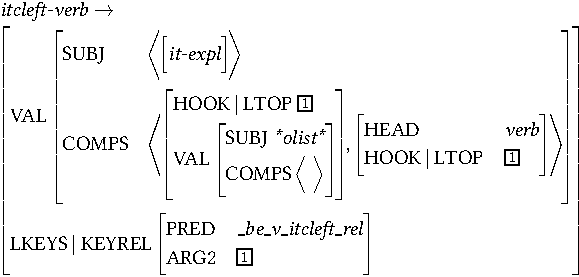
\includegraphics{pdf/itcleft-old.pdf}}}}


\myref{avm:itcleft} is my version which places several constraints on
\textit{it}-clefts in accordance with my analysis presented hitherto.


\myexe{\enumsentence{\label{avm:itcleft}
\evnup{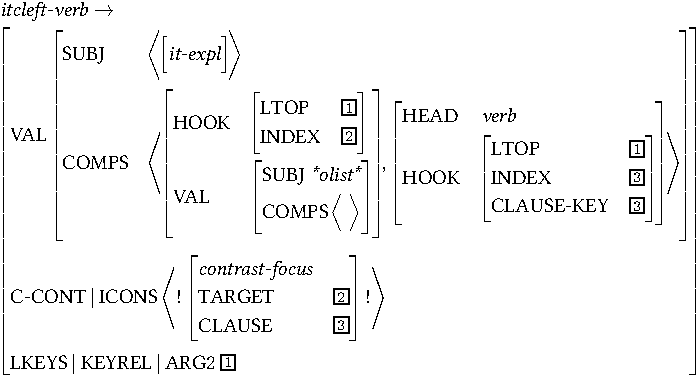
\includegraphics[width=.9\textwidth]{pdf/itcleft.pdf}}}}


\noindent The most significant difference between these two analyses
is that ICONS replaces the representation using the `discourse
relation' realized as ``\_be\_v\_itcleft\_p\_rel'' in
\myref{avm:itcleft:old}.\is{clefting} The focused XPs are assigned
\tdl{contrast-focus} within \isi{ICONS}, whose \isi{CLAUSE} value is
linked to the cleft clauses.  \myref{avm:itcleft:old} and
\myref{avm:itcleft} have the categorical restriction on the focused
XPs in common. This restriction is specified in VAL of the first
complement.  According to the corpus study \citet{kim:07} provides,
APs and VPs cannot be focused in \textit{it}-clefts as indicated in
Table~\ref{tbl:freq:cleft}, while CPs can be used as the focused XP.
Other phrasal types, such as NPs, AdvP, and PPs, can freely become the
first complement of \tdl{itcleft-verb}. This restriction is specified
using \textit{*olist*} in \mbox{VAL{$\mid$}SUBJ} and an empty list of
\mbox{VAL{$\mid$}COMPS}.


Building on the AVM in \myref{avm:itcleft},\is{clefting}
\myref{fig:clefts} exemplifies how cleft constructions are represented
via ICONS.  The information structure relation that the focused item
has to the cleft clause is analyzed as contrastive focus at least in
English due to the fact that (\ref{exe:clefts:velleman}b) and
\myref{exe:clefts:kim} sound unacceptable, though it may not hold true
cross-linguistically. Therefore, the focused element \textsc{dog} has
a \tdl{contrast-focus} relation to the cleft clause, the element
\textit{barks} in the cleft clause remains underspecified.  Note that
the expletive \textit{\mysout{it}} and the copula \textit{\mysout{is}}
are semantically empty, and thereby they cannot participate in ICONS.


\myexe{\enumsentence{\label{fig:clefts}\evnup{
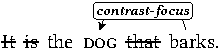
\includegraphics{pdf/clefts.pdf}}}}



\section{Passive constructions}
\label{10:sec:passive}

This section is exclusively concerned with passive constructions in
English, in order to revise the related types in the \isi{ERG} with
respect to information structure. Nonetheless, a similar version of
revision can be applied to other languages.


Passive constructions relate to the current model of information
structure in terms of two aspects; information structure and
semantics-based machine translation.\is{passive}


First, passivization is (partially) relevant to information
structure. It has been reported that some languages, such as
\ili{Spanish} \citep{casielles:03}, exhibit a relationship between
passivization and the articulation of information structure. Though
such a straightforward relationship between these concepts does not
hold for all human languages, there seems to be at least some
connection.  What is the motivation for using passive
forms?\is{passive} For this question, it is necessary to look at
promoted arguments and demoted arguments differently.  One might think
that one function of a passive is to place a different argument in
subject position so that it can be the \isi{topic} (given the general
tendency to align topic with subject). However, the promoted arguments
in passives are not always assigned \tdl{topic}. For example, the
promoted argument in the following sentence conveys a \isi{focus}
meaning, which is exclusive from a topic meaning in that the promoted
argument \textit{the book} corresponds to the \textit{wh}-word in the
question.\is{\textit{wh}-words}


\myexe{\enumsentence{\label{exe:passive:1}
\begin{tabular}[t]{ll}
Q: & {What was found by Sandy?}\\ 
A: & {The book was found by Sandy.}\\
\end{tabular}}}

 
\noindent Neither are promoted arguments always interpreted as
\tdl{focus}, because some aspect of passivization is clearly motivated
by the desire to put something other than the agent into the canonical
\isi{topic} position (i.e\ a subject position).\is{passive}

\myexe{\enumsentence{\label{exe:passive:2} They were looking all over
    for the book. Finally, it was found by Sandy.}}


\noindent As a result, the best we can say about the promoted
arguments is that they are not \isi{background}
(i.e.\ \tdl{focus-or-topic}). At the same time, the demoted arguments,
if they appear overtly, have to be marked as
\tdl{non-topic}. Particularly in English, the demoted arguments can
hardly serve as a \isi{topic} of a sentence, because NPs with
\tdl{topic} are preferentially in sentence-initial
position.\footnote{It is reported that topicalizing the demoted
  argument in passives works well in \ili{German}.\is{passive}}


Second, active/passive pairs are relevant to machine translation as
well as monolingual paraphrasing. Presumably they share the same
truth-conditions monolingually,\is{truth-conditions} and exhibit
structural divergence multilingually. For example, in English,
passives are used productively and constraints on passivization are
relatively weak. In contrast, \ili{Japanese} and \ili{Korean}, which
tend to downplay the role of passives,\is{passive} have stronger
constraints on passivization.\footnote{\citet{song:bender:11} look at
  translation of active/passive pairs to confirm how information
  structure can be used to improve transfer-based machine
  translation.} In the ERG (\textit{ver}. 1111), the passive
constructions constructionally introduce an EP (i.e.\ using C-CONT),
whose predicate is ``\_parg\_d\_rel''.  The original constraint using
the `discourse relation' is represented as follows.


\myexe{\enumsentence{\label{avm:passive:old}
\evnup{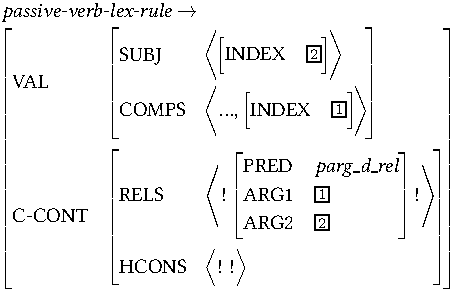
\includegraphics{pdf/passive-verb-lex-rule-old.pdf}}}}


\noindent This method cannot capture the generalization that
active/passive pairs are semantically equivalent, and does not allow
them to be paraphrased into each other monolingually. This analysis
also disregards the fact that active/passive pairs are
truth-conditionally equivalent,\is{truth-conditions} provided that the
demoted argument is overt in the passive.\is{passive} Consequently it
causes a problem in that passive sentences in English sometimes need
to be translated into active sentences in other languages, such as
Japanese and Korean. Moreover, using a discourse relation such as
``\_parg\_d\_rel'' is redundant in that this information can be provided
by an information structure value.



My alternative method is as follows. The information structure of
promoted/demoted arguments is still articulated in the lexical rule
which passivizes main verbs. However, the EP involving the discourse
predicate (i.e.\ ``parg\_d\_rel'') is removed from the lexical rule, and
instead two \tdl{info-str} values are inserted into
C-CONT.\is{\textit{info-str}} The TARGET value of the first element is
coreferenced with ARG2, and that of the second one is co-indexed with
ARG1.  In addition, the preposition \textit{by} is specified as a
semantically empty item.\is{passive} An AVM of the type responsible
for passivization is presented as \myref{avm:passive}. Note that the
first element in SUBJ and the last element in COMPS specify their
\tdl{info-str} values as \tdl{focus-or-topic} and \tdl{non-topic}
respectively.




\myexe{\enumsentence{\label{avm:passive}
\evnup{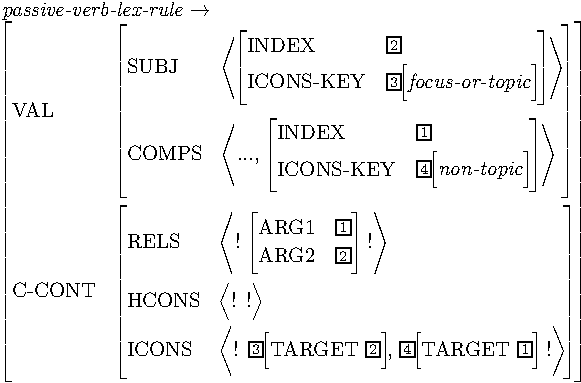
\includegraphics{pdf/passive-verb-lex-rule.pdf}}}}


\noindent A sample representation of a passive construction is
accordingly sketched out in \myref{fig:the-dog-is-chased-by-kim}, in
which the auxiliary copula \textit{\mysout{is}} and the preposition
\textit{\mysout{by}} are semantically and informatively empty.\is{passive}




\myexe{\enumsentence{\label{fig:the-dog-is-chased-by-kim}
\evnup{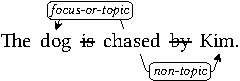
\includegraphics{pdf/the-dog-is-chased-by-kim.pdf}}}}


In the future when prosody information is modeled in the \isi{ERG} and
thereby accents for marking \isi{focus} and \isi{topic} are employed
in the grammar, the constraints on C-CONT{$\mid$}ICONS in
\myref{avm:passive} should be changed. If rules for dealing with
prosody are used, the rules will be responsible for introducing the
\isi{ICONS} elements for constraining information structure values on
promoted and demoted arguments. In this case,\is{ICONS-KEY}
\tdl{passive-verb-lex-rule} will have an empty C-CONT{$\mid$}ICONS,
but it still will assign specific values to the ICONS-KEYs of the
promoted arguments (\tdl{focus-or-topic} on the first element of SUBJ)
and demoted arguments (\tdl{non-topic} on the last element of
COMPS). Because prosodic information has not yet been used in the
current ERG, tentatively \myref{avm:passive} puts the \isi{ICONS}
elements into C-CONT herein.



\section{Fronting}
\label{10:sec:fronting}



\myref{exe:the-book-kim-reads} exemplifies a \isi{focus}/\isi{topic}
\isi{fronting} construction in English:
(\ref{exe:the-book-kim-reads}a) is the unmarked sentential form which
is devoid of any specific information structure markings. On the other
hand, the object \textit{the book} in (\ref{exe:the-book-kim-reads}b)
occupies the sentence-initial position, and the remaining part of the
sentence has a syntactic gap for the preposed object.

\myexe{\eenumsentence{\toplabel{exe:the-book-kim-reads}
\item Kim reads the book.
\item The book Kim reads.}}



The point at issue in analyzing \isi{focus}/\isi{topic} fronting
constructions is to determine which information structure meaning(s)
the preposed argument gives. (\ref{exe:the-book-kim-reads}b) in itself
sounds ambiguous between two possible readings: One assigns a topic
reading to \textit{the book}, and bears a likeness to an \textit{`as
  for ...'}  construction. The other, similarly to \textit{it}-clefts,
has a focus reading on the preposed argument. The choice between them
is largely conditioned by the contextual situation that utterances
prior to the current sentence create, which is infeasible to measure
in sentence-based language processing \citep{kuhn:96}. Thus, as long
as we do not deploy an extra device to resolve the meaning with
respect to the context, the information structure value on \textit{the
  book} should be underspecified so that it can cover both
meanings.\is{\textit{info-str}} The lowest supertype of both
\tdl{focus} and \tdl{topic} in Figure~\ref{fig:info-str} is
\tdl{focus-or-topic}, which implies the associated constituents
(e.g.\ \textit{the book} in \ref{exe:the-book-kim-reads}b) are
informatively interpreted as either focus or
\isi{topic}. \myref{fig:the-book-kim-reads:1} is illustrative of the
schema that (\ref{exe:the-book-kim-reads}b) has.




\myexe{\enumsentence{\label{fig:the-book-kim-reads:1}\evnup{
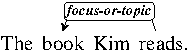
\includegraphics{pdf/the-book-kim-reads-1.pdf}}}}



\section{Dislocation}
\label{10:sec:dislocation}


Unlike \isi{focus}/\isi{topic} \isi{fronting} constructions,
\isi{dislocation} constructions do not have any syntactic gap
irrespective of whether the peripheral topic is sentence-initial
(i.e.\ \isi{left dislocation}) or sentence-final (i.e.\ \isi{right
  dislocation}).\is{periphery} The example structurally similar to
(\ref{exe:the-book-kim-reads}b) is provided in
\myref{exe:the-book-kim-reads-it}\footnote{Commas after topicalized
  NPs are not obligatorily used, and are mainly attached just as a
  preferable writing style for the reader's convenience.  On the other
  hand, there should be a phonetic pause between the topicalized NPs
  and the main sentence in speech. The pause information should be
  included in the typed feature structure of PHON, because information
  structure-based \isi{TTS} (Text-To-Speech) and ASR (Automatic Speech
  Recognition) systems can use it to improve performance.}, in which
(i) an intonational break at the phonological level intervenes between
the left-peripheral NP \textit{the book} and the rest of the
utterance, and (ii) a resumptive pronoun \textit{it} corresponding to
\textit{the book} satisfies the object of \textit{reads}.


\myexe{\eenumsentence{\toplabel{exe:the-book-kim-reads-it}
\item The book, Kim reads it.
\item Kim reads it, the book.}}

\textit{The book} in this case is an external \isi{topic} that is not
inside the sentence. It is regarded as containing \tdl{frame-setting}
information according to the cross-linguistic study offered in the
previous chapters. In other words, its pragmatic role is to narrow the
domain of what is being referred to.\is{frame-setting}



In the analysis of \isi{dislocation}, there is one more factor to be
considered; agreement between the topicalized NP and the corresponding
pronoun inside the head sentence. For example, in
\myref{exe:the-book-kim-reads-it} only the third singular pronoun
\textit{it} which agrees with \textit{the book} can be resumptive. In
languages which exhibit rich morphology (e.g.\ \ili{Italian}
\citep{cinque:77,rizzi:97}, \ili{Spanish}
\citep{rivero:80,zagona:02,bildhauer:08}, \ili{German}
\citep{grohmann:01}, Modern \ili{Greek}
\citep{alexopoulou:kolliakou:02}, \ili{Czech} \citep{sturgeon:10},
etc.) the choice of resumptive pronouns matters. The options are: (i)
(clitic) left dislocations and (ii) hanging topics. The resumptive
pronouns in left dislocation constructions have to agree perfectly
with the dislocated NP in person, number, gender, case, etc., whereas
a hanging \isi{topic} and its corresponding pronoun do not agree with
each other.  This implies that hanging topics have a looser
relationship with the remaining part of the sentence than left
dislocations \citep{frascarelli:00}.\is{left dislocation}\is{hanging
  topic}



\myexe{\eenumsentence{\label{exe:clld:haning-topic}
\item\shortex{5}
{[Seinen$_{i}$ & Vater], & den & mag & jeder$_{i}$.}
{his-\textsc{acc} & father & \textsc{rp-acc} & likes & everyone}
{`His father, everyone likes.'}
\item\shortex{5}
{[Sein$_{i}$ & Vater], & jeder$_{*i/k}$ & mag & den/ihn.}
{his-\textsc{nom} & father & everyone & likes & \textsc{rp}/him-\textsc{acc}}
{`His father, everyone likes him.' [ger] \citep[92]{grohmann:01}}
\item\shortex{4}
{Honzu, & toho & j\v{e}st\v{e} & nezn\'{a}m.}
{Honza.\textsc{acc} & that.\textsc{acc} & still & \textsc{neg}-know.\textsc{1sg}}
{`Honza, I still don't know him.'}
\item\shortex{5}
{Ani\v{c}ka? & T\'{e} & se & nic & nestalo.}
{Ani\v{c}ka.\textsc{nom} & that.\textsc{dat} & \textsc{refl-cl} & nothing & \textsc{neg}-happened}
{`Ani\v{c}ka? Nothing happened to her.' [cse] \citep[288]{sturgeon:10}}}}



\noindent (\ref{exe:clld:haning-topic}a--b) are examples of left
dislocation and hanging topics in \ili{German}, respectively.  In
(\ref{exe:clld:haning-topic}a), the accusative on the dislocated NP
\textit{Seinen Vater} agrees with that on the resumptive pronoun
\textit{den}. By contrast, a hanging topic \textit{Sein Vater} in
(\ref{exe:clld:haning-topic}b) is in nominative, which does not agree
with the resumptive pronoun in accusative. The same holds for
(\ref{exe:clld:haning-topic}c--d) in \ili{Czech}; both \textit{Honza}
and its resumptive pronoun \textit{toho} in
(\ref{exe:clld:haning-topic}c) are in accusative, while there is no
agreement between the lefthand NP \textit{Ani\v{c}ka} and
\textit{T\'{e}} in (\ref{exe:clld:haning-topic}d).


In movement-based analyses, (clitic) left dislocations and hanging
topics are regarded as being configured via two different syntactic
operations: Dislocated NPs in (clitic) left dislocations are
originally realized inside the sentence, and move forward leaving
resumptive pronouns with the same features. Hanging topics, by
contrast, are base-generated \textit{ab initio} without any agreement
with their corresponding pronoun.\is{hanging topic} Hanging topics in
transformation-based studies are also assumed to have several
additional characteristics \citep{frascarelli:00}: (i) Only one
hanging \isi{topic} can show up in a sentence, (ii) hanging topics can
appear only sentence-initially, (iii) if a hanging topic co-occurs
with other topics in a sentence, it should be followed by the other
topics (i.e.\ hanging topic first).\footnote{\citet{frascarelli:00},
  exploiting a corpus, provides some counterexamples to these
  properties that hanging topics presumably possess, which implies
  they are tendencies, rather than strict rules.}  From this point of
view, \cite{cinque:77} distinguishes English-like languages from
Italian-like languages.\il{English}\il{Italian} The former employ only
hanging topics, whereas the latter have both left dislocation and
hanging topics.\is{left dislocation}


In \isi{HPSG}-based studies, agreement between a dislocated NP and its
resumptive pronoun is modeled. For instance, in the following AVM
taken from \citet[350]{bildhauer:08}, a coreference \fbox{3} means
the HEAD-values should be consistent in order to capture
case-agreement, and another coreference \fbox{4} indicates that they
share the same INDEX.

\myexe{\enumsentence{\label{avm:clld-phrase-bildhauer}\evnup{
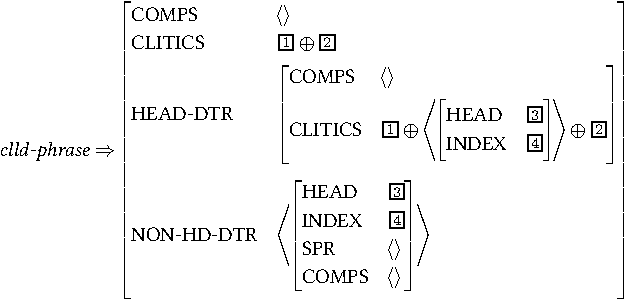
\includegraphics[width=.9\textwidth]{pdf/clld-phrase-bildhauer.pdf}}}}


Because the present study does not employ a rigid distinction between
(clitic) left dislocations and hanging topics, all these constraints
can be fully covered in the current proposal. That is,
they can be merged into just one single type that assigns
\tdl{contrast-topic} to the fronted constituent. 



\myexe{\enumsentence{\label{fig:dislocation}
\begin{tabular}[t]{lllll}
a. & \evnup{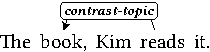
\includegraphics{pdf/left-dislocation.pdf}} & & b. &
\evnup{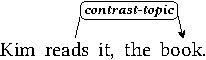
\includegraphics{pdf/right-dislocation.pdf}} \\
\end{tabular}}}


As mentioned earlier, the present work does not fully implement
\isi{focus}/\isi{topic} \isi{fronting} and \isi{dislocation} in terms
of how to build up this representation compositionally. In
Section \ref{11:ssec:phr}, several types of dislocated constituents are
partially implemented using \tdl{head-filler-phrase} in order to
constrain clause-initial and clause-final foci. Future work needs to
look into how the \tdl{contrast-topic} element can be added into the
\isi{ICONS} list.





\section{Summary}
\label{10-4:sec:summary}


This chapter has delved into the specific forms of expressing
information structure. First, \isi{focus} sensitive items are
classified into two subtypes;\is{focus sensitive item} one assigns an
information structure value to itself, and the other assigns a value
to its adjacent item.  Second, in terms of argument
optionality,\is{argument optionality} unexpressed arguments always
bear \tdl{non-focus} because focused items cannot be elided. Third,
scrambling in \ili{Japanese} and \ili{Korean} was addressed. The
present study proposes a cross-classification of three phrase
structure types, which refer to an MKG value for looking at which
lexical marker is used.\is{MKG}\is{lexical markers} Fourth, an AVM
responsible for cleft constructions in the \isi{ERG} was revised to
signal \tdl{focus} (i.e.\ a plain focus) to the pivot XP in cleft
constructions.  Fifth, promoted and demoted arguments in passive
constructions also have a specific \tdl{info-str}
value:\is{\textit{info-str}} \tdl{focus-or-topic} for the former, and
\tdl{non-topic} for the latter.  Lastly, focus/\isi{topic}
\isi{fronting} constructions and two types of dislocations
(i.e.\ left dislocation and hanging topics) were
examined. The fronted elements in OSV sentences in English have a
value of \tdl{focus-or-topic}, because they can be interpreted as
either \tdl{focus} or \tdl{topic}.\is{focus sensitive item} On the
other hand, dislocated NPs are assigned \tdl{contrast-topic} in line
with the analyses of previous studies.\is{dislocation}



